\chapter{Anwendungen von DFS}

\section{Starke Zusammenhangskomponenten}

\term{Zusammenhangskomponenten}\index{Zusammenhangskomponente} in einem ungerichteten Graph sind Teilgraphen, in denen es zwischen je zwei beliebigen Knoten einen Pfad gibt.

In gerichteten Graphen sind \term{starke Zusammenhangskomponenten}\index{Zusammenhangskomponente!stark} Teilgraphen \( G \subseteq H \), in denen ebenfalls gilt: für jedes Knotenpaar \( u,v \in G \) gibt es einen \( u \)-\( v \)-Pfad \emph{und} einen \( v \)-\( u \)-Pfad.

Insbesondere werden starke Zusammenhangskomponenten durch Zyklen erzeugt (dann kann man einfach im Kreis laufen von einem Knoten zum anderen). Das bedeutet im Umkehrschluss, dass der \term{Schrumpfgraph}\index{Schrumpfgraph} --- das ist der Graph, den man erhält, indem man jede starke Zusammenhangskomponente als einen Knoten zusammenfasst --- zyklenfrei ist.

\begin{figure}[H]
  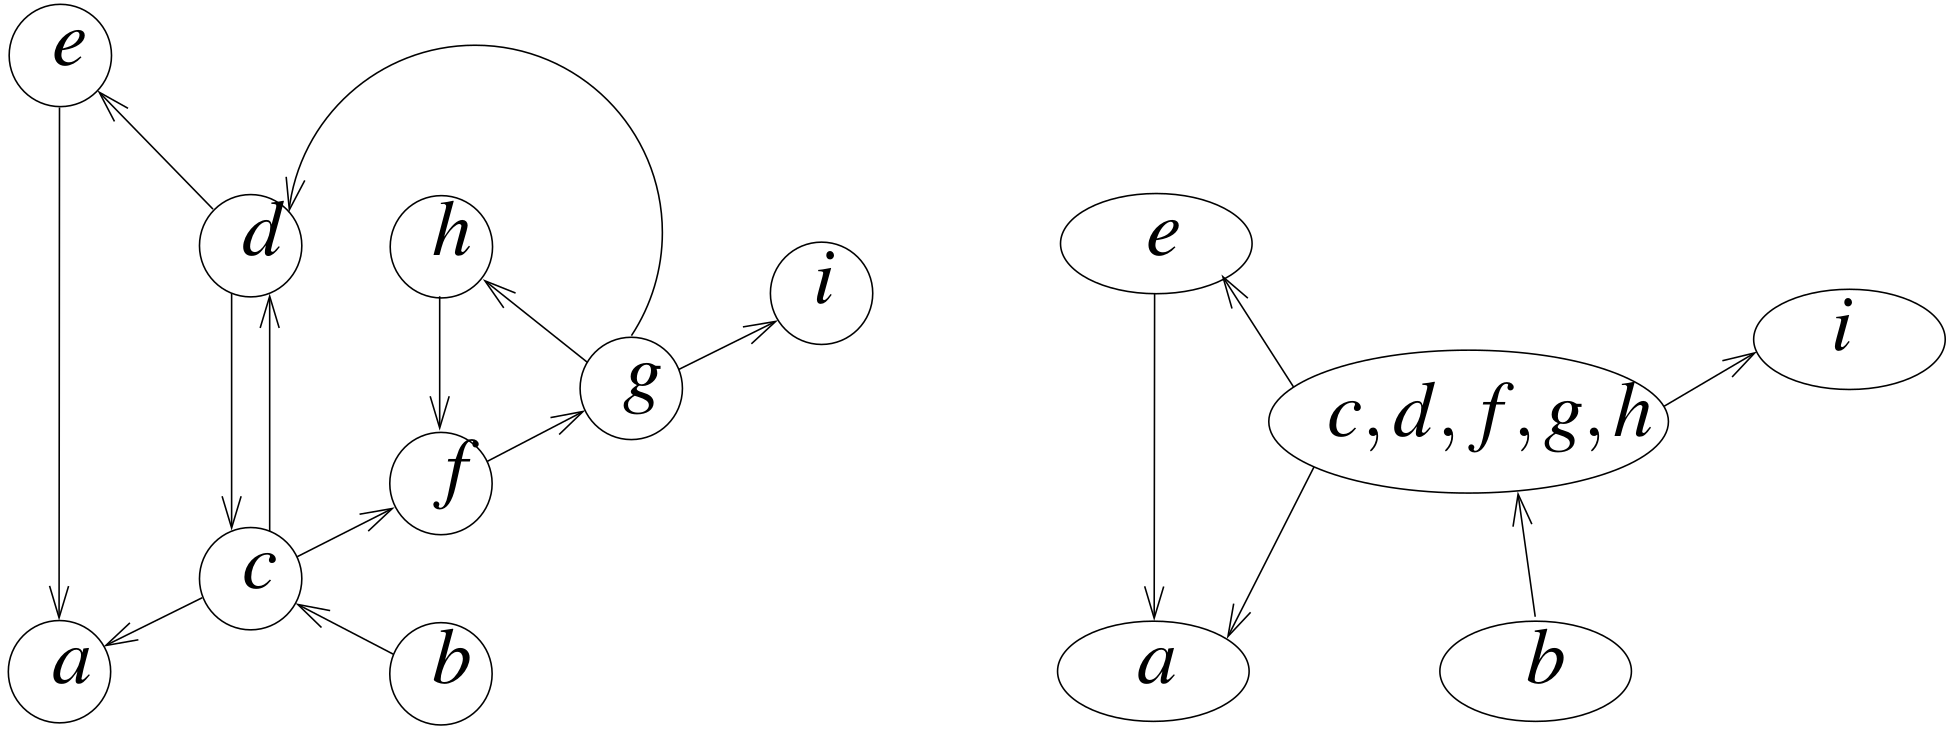
\includegraphics[width=0.6\textwidth]{schrumpfgraph}
  \caption{Gerichteter Graph \( G \) und zugehöriger Schrumpfgraph \( G_S \)}
\end{figure}

\subsection{Tiefensuchschema}

Um später SCCs ermitteln zu können konstruieren wir ein Tiefensuchschema:

\begin{pseudocode}
  unmark all nodes \\
  \textcolor{red}{init}\( () \) \\
  \textbf{foreach} \( s \in V \) \textbf{do} \\
  \phantom{\enskip} \textbf{if} \( s \) is not marked \textbf{then} \\
  \phantom{\enskip} \phantom{\enskip} mark s \\
  \phantom{\enskip} \phantom{\enskip} \textcolor{red}{root}\( (s) \) \\
  \phantom{\enskip} \phantom{\enskip} DFS\( (s,s) \) \\
  \ \\
  \textbf{\textsc{DFS}}\( (u,v : \text{Node}) \) \\
  \phantom{\enskip} \textbf{foreach} \( (v,w) \in E \) \textbf{do} \\
  \phantom{\enskip} \phantom{\enskip} \textbf{if} \( w \) is marked \textbf{then} \\ \phantom{\enskip} \phantom{\enskip} \phantom{\enskip} \textcolor{red}{traverseNonTreeEdge}\( (v,w) \) \\
  \phantom{\enskip} \phantom{\enskip} \textbf{else} \\
  \phantom{\enskip} \phantom{\enskip} \phantom{\enskip} \textcolor{red}{traverseTreeEdge}\( (v,w) \) \\
  \phantom{\enskip} \phantom{\enskip} \phantom{\enskip} mark w \\
  \phantom{\enskip} \phantom{\enskip} \phantom{\enskip} DFS\( (v,w) \) \\
  \phantom{\enskip} \textcolor{red}{backtrack}\( (u,v) \)
\end{pseudocode}

Dieses Tiefensuchschema kann auf unterschiedliche Graphtraversierungsprobleme angepasst werden.

Wir verwenden nun zwei Arrays zum Zwischenspeichern unserer Resultate:
\begin{itemize}
  \item \code{oNodes} speichert die bereits besuchten Knoten,
  \item \code{oReps} speichert die Repräsentanten der einzelnen SCCs.
\end{itemize}

Beim Durchlaufen des Graphen werden die Knoten mit \code{dfsNum} inkrementell durchnummeriert.

Außerdem gibt es drei Invarianten, die wir im Folgenden nicht verletzen dürfen:
\begin{enumerate}
  \item Kanten von abgeschlossenen Knoten gehen zu abgeschlossenen Knoten
  \item Offene Komponenten \( S_1,\dots,S_k \) bilden einen Pfad in \( G_C^s \).
  \item Repräsentanten partitionieren die offenen Komponenten bezüglich ihrer \code{dfsNum}.
\end{enumerate}

Für das Finden von SCCs brauchen wir folgende Implementierungen für die rot gekennzeichneten Prozesuren:
\begin{itemize}
  \item \textbf{\code{root(s)}}:
  \begin{pseudocode}
    oReps.push\( (s) \) \\
    oNodes.push\( (s) \)
  \end{pseudocode}
  Hierdurch wird eine neue offene Komponente gebildet und \( s \) als besucht gekennzeichnet.

  \item \textbf{\code{traverseTreeEdge(v,w)}}:
  \begin{pseudocode}
    oReps.push\( (w) \) \\
    oNodes.push\( (w) \)
  \end{pseudocode}
  Hier wird \( \left \{ w \right \} \) als neue offene Komponente angelegt.

  \item \textbf{\code{traverseNonTreeEdge(v,w)}}:
  \begin{pseudocode}
    \textbf{if} \( w \in \text{oNodes} \) \textbf{then} \\
    \phantom{\enskip} \textbf{while} \( w\text{.dfsNum} < \text{oReps.top.dfsNum} \) \textbf{do} oReps.pop
  \end{pseudocode}
  Ist \( w \not \in \text{oNodes} \) ist \( w \) abgeschlossen und die Kante somit uninteressant. Ist \( w \) allerdings in oNodes, so werden die auf dem Kreis befindlichen SCCs kollabiert.

  \item \textbf{\code{backtrack(u,v)}}:
  \begin{pseudocode}
    \textbf{if} \( v \equiv \text{oReps.top} \) \textbf{then} \\
    \phantom{\enskip} \text{oReps.pop} \\
    \phantom{\enskip} \textbf{repeat} \\
    \phantom{\enskip} \phantom{\enskip} \( w \coloneqq \text{oNodes.pop} \) \\
    \phantom{\enskip} \phantom{\enskip} \( \text{component}[w] \coloneqq v \) \\
    \phantom{\enskip} \textbf{until} \( w = v \)
  \end{pseudocode}
\end{itemize}

Damit haben wir alles was wir brauchen, um die Suche nach SCCs durchführen zu können. Wir kriegen sie sogar in \( O(m+n) \), also in Linearzeit, hin!

\begin{figure}[H]
  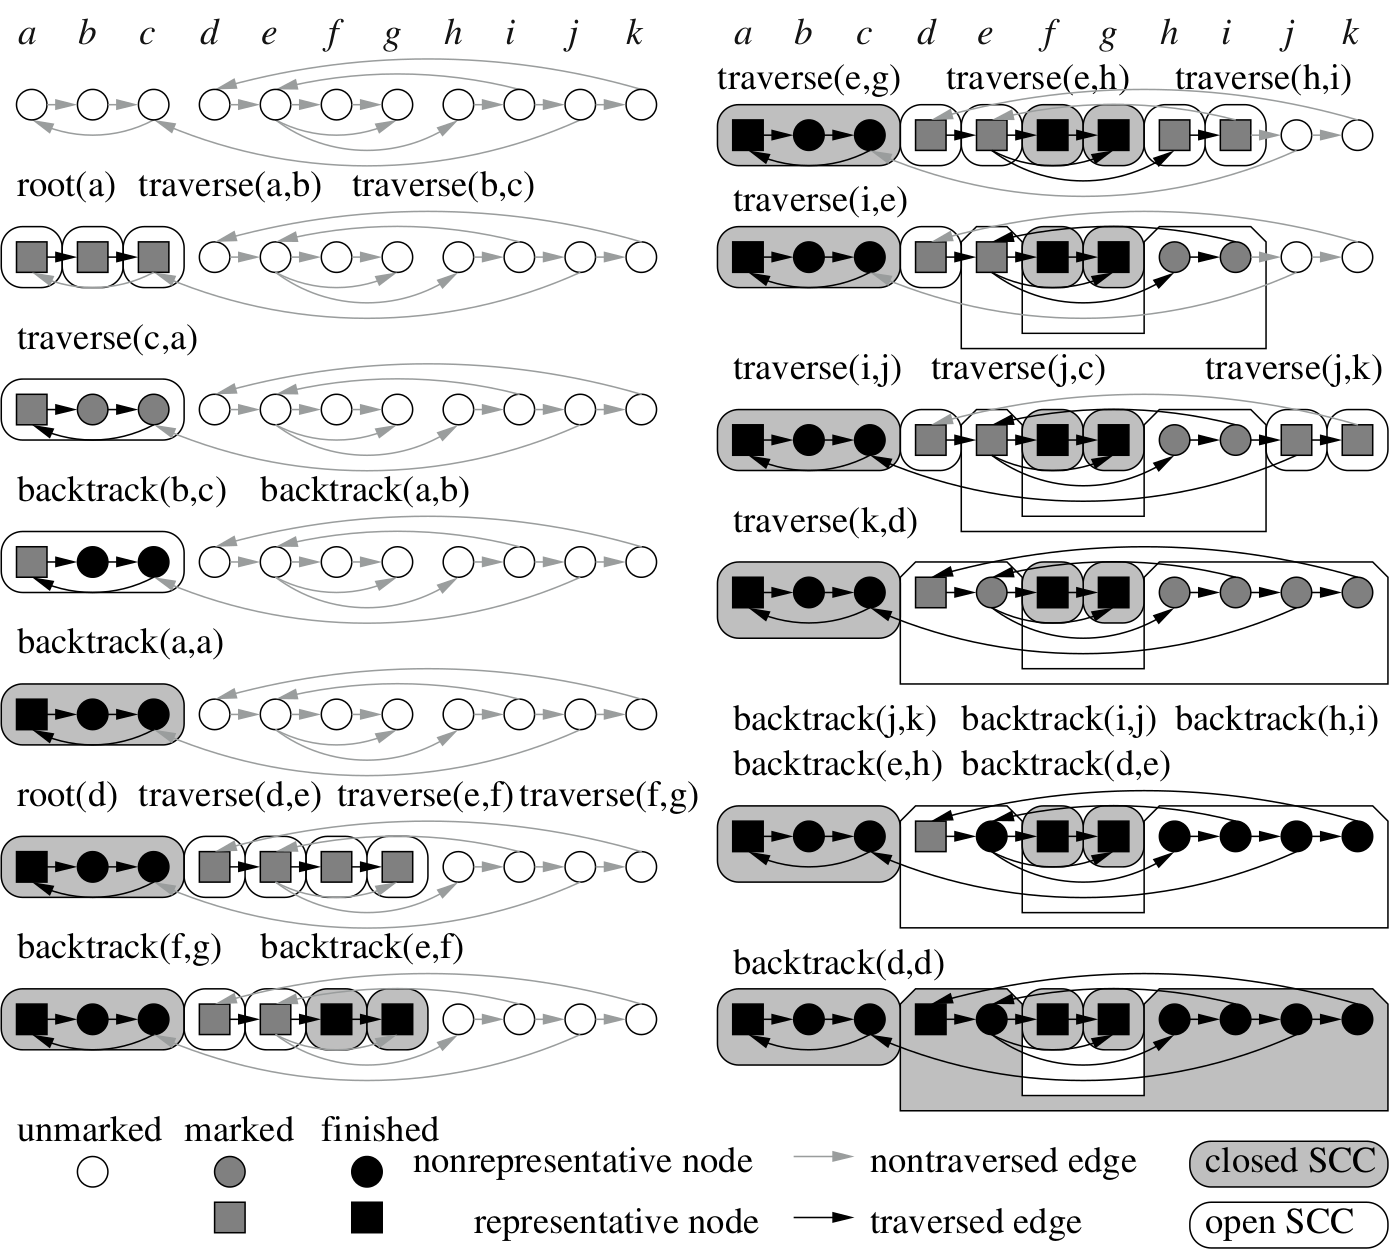
\includegraphics[width=0.6\textwidth]{SCC}
  \caption{Kompletter Durchlauf des Algorithmus}
\end{figure}